\documentclass[10pt,a4paper]{article}

\usepackage{etex} % расширение классического tex в частности позволяет подгружать гораздо больше пакетов, чем мы и займёмся далее

%%%%%%%%%% Математика %%%%%%%%%%
\usepackage{amsmath,amsfonts,amssymb,amsthm,mathtools}
%\mathtoolsset{showonlyrefs=true}  % Показывать номера только у тех формул, на которые есть \eqref{} в тексте.
%\usepackage{leqno} % Нумерация формул слева
\usepackage{color,colortbl}
\definecolor{lightRed}{RGB}{230,170,150}
\definecolor{LightCyan}{rgb}{0.88,1,1}
\definecolor{lightGray}{gray}{0.9}
\usepackage[table]{xcolor}
\usepackage{colortbl}
\setlength\arrayrulewidth{2pt}


%%%%%%%%%%%%%%%%%%%%%%%% Шрифты %%%%%%%%%%%%%%%%%%%%%%%%%%%%%%%%%

\usepackage{fontspec}         % пакет для подгрузки шрифтов
\setmainfont{Arial}   % задаёт основной шрифт документа

\defaultfontfeatures{Mapping=tex-text}

% why do we need \newfontfamily:
% http://tex.stackexchange.com/questions/91507/
\newfontfamily{\cyrillicfonttt}{Arial}
\newfontfamily{\cyrillicfont}{Arial}
\newfontfamily{\cyrillicfontsf}{Arial}

\usepackage{unicode-math}     % пакет для установки математического шрифта
\setmathfont{Asana-Math.otf}      % шрифт для математики

\usepackage{polyglossia}      % Пакет, который позволяет подгружать русские буквы
\setdefaultlanguage{russian}  % Основной язык документа
\setotherlanguage{english}    % Второстепенный язык документа



%%%%%%%%%% Работа с картинками %%%%%%%%%
\usepackage{graphicx}                  % Для вставки рисунков
\usepackage{graphics}
\graphicspath{{images/}{pictures/}}    % можно указать папки с картинками
\usepackage{wrapfig}                   % Обтекание рисунков и таблиц текстом
\usepackage{subfigure}                 % для создания нескольких рисунков внутри одного


%%%%%%%%%% Работа с таблицами %%%%%%%%%%
\usepackage{tabularx}            % новые типы колонок
\usepackage{tabulary}            % и ещё новые типы колонок
\usepackage{array}               % Дополнительная работа с таблицами
\usepackage{longtable}           % Длинные таблицы
\usepackage{multirow}            % Слияние строк в таблице
\usepackage{float}               % возможность позиционировать объекты в нужном месте
\usepackage{booktabs}            % таблицы как в книгах!
\renewcommand{\arraystretch}{1.3} % больше расстояние между строками



% Незнакомые нам команды :)
\DeclareMathOperator{\diag}{diag}  % математический оператор, который описывает диагональную матрицу

\usepackage[landscape,top=2mm, bottom=2mm,left=2mm,right=2mm,includefoot]{geometry}
% Параметры страницы. Сколько надо делать и где поля. Обсудим его подробнее через одну неделю ;)


\begin{document}
\pagestyle{empty}


\begin{table}
\begin{tabularx}{\textwidth}{|p{0.1\linewidth}|p{0.13\linewidth}|p{0.07\linewidth}|p{0.05\linewidth}|p{0.16\linewidth}|p{0.53\linewidth}}

\rowcolor{LightCyan} Метод & Оценка & Год\newline создания & Автор & Фотка автора & Описание \\

\hline
\rowcolor{lightGray}Метод наименьших квадратов (OLS) & \[(X^{T}X)^{-1}X^Ty\] & 1795 & \textdegree Carl Friedrich Gauss \newline \textdegree Лежандр &   \center{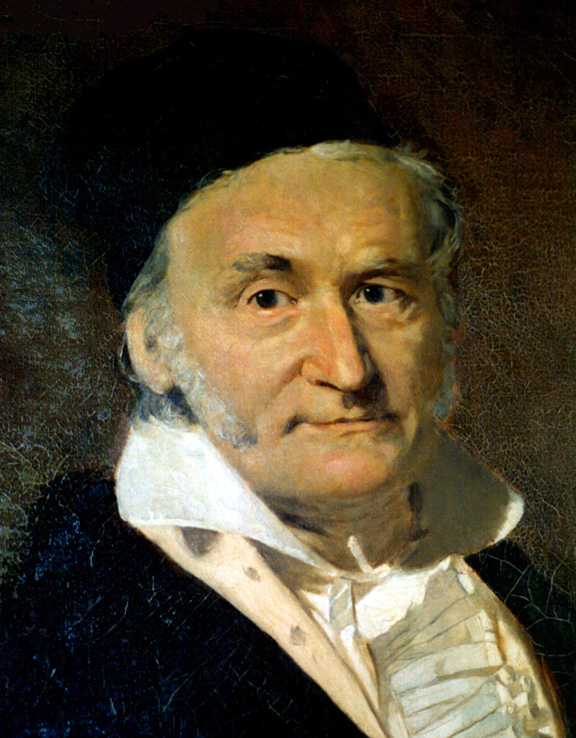
\includegraphics[width=0.3\linewidth]{gauss.jpg}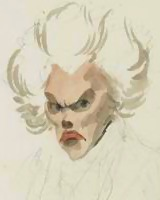
\includegraphics[width=0.3\linewidth]{lezhandr.jpg}    } & Метод оценивания параметров эконометрической модели,\newline состоящий в минимизации суммы квадратов расхождений между \newline наблюдаемыми значениями зависимой переменной и значениями \newline этой переменной, вычисленными для наблюдаемых значений\newline независимых переменных  по оценённой модели связи. \\

\hline

\rowcolor{lightGray}Обобщённый метод наименьших квадратов (GLS) &  \[(X^T \Omega^{-1} X)^{-1}X^T \Omega^{-1} y\] & 1934 & Alexander Aitken & \center{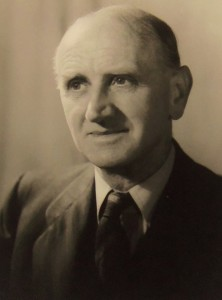
\includegraphics[width=0.3\linewidth]{aitken1.jpg}}  & Теоретическая процедура оценивания коэффициентов линейной \newline модели регрессии в ситуации, когда случайные ошибки имеют \newline разные дисперсии и коррелированы между собой, при этом \newline предполагается,  что ковариационная матрица вектора ошибок \newline невырождена и все ее элементы известны. \\
\hline
\rowcolor{lightGray}Взвешенный метод наименьших квадратов (WLS) &  \[ (X^T \Omega^{-1} X)^{-1}  X^T \Omega^{-1} y\] при этом \newline $\Omega = \diag(\sigma_1,\sigma_2, \ldots \sigma_n) $ &  он же & он же & он же  & Процедура, состоящая в минимизации определённым образом \newline взвешенной суммы квадратов отклонений наблюдаемых значений\newline зависимой переменной от значений, вычисляемых по подбираемой\newline модели связи. \\

\hline

\rowcolor{lightGray}Доступный обобщённый метод наименьших квадратов (FGLS) & \[(X^T \hat{\Omega}^{-1} X)^{-1}X^T \hat{\Omega}^{-1} y\] & тот же & он же & он же & Практически реализуемая процедура оценивания коэффициентов \newline линейной модели регрессии в ситуации, когда случайные ошибки \newline имеют разные дисперсии и коррелированы между собой,\newline повторяющая процедуру обобщенного метода наименьших \newline квадратов, но использующая оцененную ковариационную матрицу \newline вектора ошибок. \\
\hline
\rowcolor{lightGray}Косвенный метод наименьших квадратов (ILS) & & В 1928 начали заниматься проблемой инструментальных переменных  & \textdegree Philip Wright \newline \textdegree Sewall Wright \newline (отец и сын)& \center{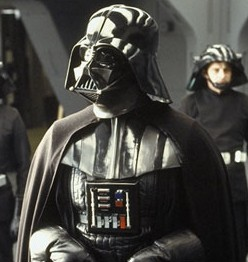
\includegraphics[width=0.36\linewidth]{Darth_Vader.jpg}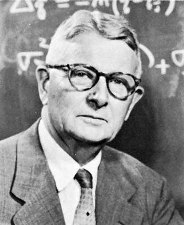
\includegraphics[width=0.3\linewidth]{Sewall_Wright.jpg}}  & метод получения оценок параметров $i-$го стохастического \newline уравнения структурной формы через оценки наименьших квадратов \newline коэффициентов уравнений приведенной формы. Метод применим в \newline случае точной идентифицируемости $i-$го структурного уравнения.\\

\hline

\rowcolor{lightGray}Двухшаговый метод наименьших квадратов (2SLS) & \begin{multline*}(X^T Z (Z^T Z)^{-1} Z^T X)^{-1}\cdot \\ \cdot X^T Z(Z^T Z)^{-1} Z^Ty \end{multline*} & 1953 \newline   1957 & \textdegree Henri Theil \newline \textdegree Robert Basmann & \center{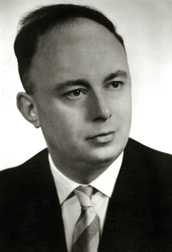
\includegraphics[width=0.27\linewidth]{theil1.jpg}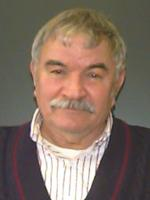
\includegraphics[width=0.3\linewidth]{basmann.jpg}    }  &  Метод оценивания коэффициентов уравнения структурной формы,\newline состоящий в предварительной очистке стохастической объясняющей \newline переменой от коррелированности с ошибкой в этом уравнении с \newline использованием инструментальных переменных и в последующем \newline  оценивании уравнения, в котором исходная объясняющая\newline переменная заменяется ее очищенным вариантом. \\
\hline
\rowcolor{lightGray}Трёхшаговый метод наименьших квадратов (3SLS) & \begin{multline*} (\hat Z^T(\hat \Lambda^{-1} \otimes I_g) \hat Z)^{-1}\cdot \\ \cdot \hat Z^T (\hat \Lambda^{-1} \otimes I_g)y \end{multline*} & они же & они же & они же & Доступный обобщённый метод наименьших квадратов, применённый \newline к системе одновременных уравнений. Принимает во внимание наличие \newline коррелирванности между ошибками в разных структурных \newline уравнениях. \\
\hline
\end{tabularx}
\end{table}

\end{document}
